
\begin{figure}[!t]
\begin{center}
  \begin{footnotesize}
\subfigure[Regular Events]{
    \label{fig:event_storage_fxt}
    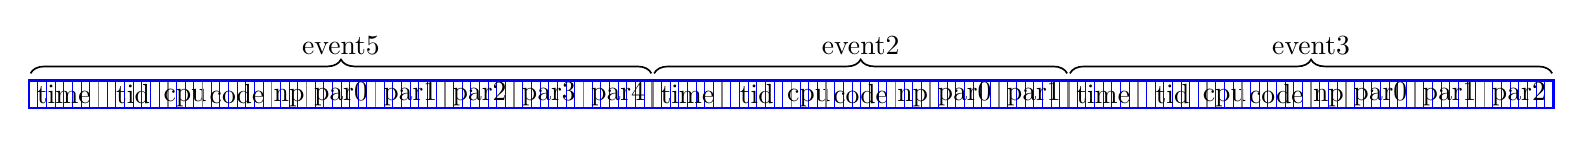
\begin{tikzpicture}[scale=.88]
    % vertical lines
    \foreach \x in {.125,.25,...,21.875}
        \draw[blue,line width=.12mm](\x,1.2) -- (\x,1.6);gray
    % event5
    \draw [
    semithick,
    decorate,
    decoration={
        brace,
        amplitude=5pt,
        raise=-0.35cm
    }] (0.02,2.1) -- (8.98, 2.1) node[midway]{event5}; 
    \draw (0.5, 1.4) -- (0.5, 1.4) node{time};
    \draw[gray,line width=.2mm](1.,1.2) -- (1.,1.6);
    \draw (1.5, 1.4) -- (1.5, 1.4) node{tid};
    \draw[gray,line width=.2mm](2.,1.2) -- (2.,1.6);
    \draw (2.25, 1.35) -- (2.25, 1.35) node{cpu};
    \draw[gray,line width=.2mm](2.5,1.2) -- (2.5,1.6);  
    \draw (3., 1.4) -- (3., 1.4) node{code};
    \draw[gray,line width=.2mm](3.5,1.2) -- (3.5,1.6);
    \draw (3.75, 1.35) -- (3.75, 1.35) node{np};
    \draw[gray,line width=.2mm](4.,1.2) -- (4.,1.6);    
    \draw (4.5, 1.4) -- (4.5, 1.4) node{par0};
    \draw[gray,line width=.2mm](5.,1.2) -- (5.,1.6);
    \draw (5.5, 1.4) -- (5.5, 1.4) node{par1};
    \draw[gray,line width=.2mm](6.,1.2) -- (6.,1.6);
    \draw (6.5, 1.4) -- (6.5, 1.4) node{par2};
    \draw[gray,line width=.2mm](7.,1.2) -- (7.,1.6);  
    \draw (7.5, 1.4) -- (7.5, 1.4) node{par3};
    \draw[gray,line width=.2mm](8.,1.2) -- (8.,1.6);
    \draw (8.5, 1.4) -- (8.5, 1.4) node{par4};
    \draw[gray,line width=.4mm](9.,1.2) -- (9.,1.6);    
    % event2
    \draw [
    semithick,
    decorate,
    decoration={
        brace,
        amplitude=5pt,
        raise=-0.35cm
    }] (9.02,2.1) -- (14.98, 2.1) node[midway]{event2};     
    \draw (9.5, 1.4) -- (9.5, 1.4) node{time};
    \draw[gray,line width=.2mm](10.,1.2) -- (10.,1.6);
    \draw (10.5, 1.4) -- (10.5, 1.4) node{tid};
    \draw[gray,line width=.2mm](11.,1.2) -- (11.,1.6);
    \draw (11.25, 1.35) -- (11.25, 1.35) node{cpu};
    \draw[gray,line width=.2mm](11.5,1.2) -- (11.5,1.6);  
    \draw (12., 1.4) -- (12., 1.4) node{code};
    \draw[gray,line width=.2mm](12.5,1.2) -- (12.5,1.6);
    \draw (12.75, 1.35) -- (12.75, 1.35) node{np};
    \draw[gray,line width=.2mm](13.,1.2) -- (13.,1.6);
    \draw (13.5, 1.4) -- (13.5, 1.4) node{par0};
    \draw[gray,line width=.2mm](14.,1.2) -- (14.,1.6);    
    \draw (14.5, 1.4) -- (14.5, 1.4) node{par1};
    \draw[gray,line width=.4mm](15.,1.2) -- (15.,1.6);    
    % event3
    \draw [
    semithick,
    decorate,
    decoration={
        brace,
        amplitude=5pt,
        raise=-0.35cm
    }] (15.02,2.1) -- (21.98, 2.1) node[midway]{event3};         
    \draw (15.5, 1.4) -- (15.5, 1.4) node{time};
    \draw[gray,line width=.2mm](16.,1.2) -- (16.,1.6);
    \draw (16.5, 1.4) -- (16.5, 1.4) node{tid};
    \draw[gray,line width=.2mm](17.,1.2) -- (17.,1.6);
    \draw (17.25, 1.35) -- (17.25, 1.35) node{cpu};
    \draw[gray,line width=.2mm](17.5,1.2) -- (17.5,1.6);  
    \draw (18., 1.4) -- (18., 1.4) node{code};
    \draw[gray,line width=.2mm](18.5,1.2) -- (18.5,1.6);
    \draw (18.75, 1.35) -- (18.75, 1.35) node{np};
    \draw[gray,line width=.2mm](19.,1.2) -- (19.,1.6);
    \draw (19.5, 1.4) -- (19.5, 1.4) node{par0};
    \draw[gray,line width=.2mm](20.,1.2) -- (20.,1.6);    
    \draw (20.5, 1.4) -- (20.5, 1.4) node{par1};
    \draw[gray,line width=.2mm](21.,1.2) -- (21.,1.6);    
    \draw (21.5, 1.4) -- (21.5, 1.4) node{par2};
    % big rectangle
    \draw [blue, line width=.3mm]
        (0.,1.2) rectangle (22.,1.6);
           
    \end{tikzpicture}
}
\subfigure[Packed Events]{
    \label{fig:event_storage_litl}
    \hspace*{2mm}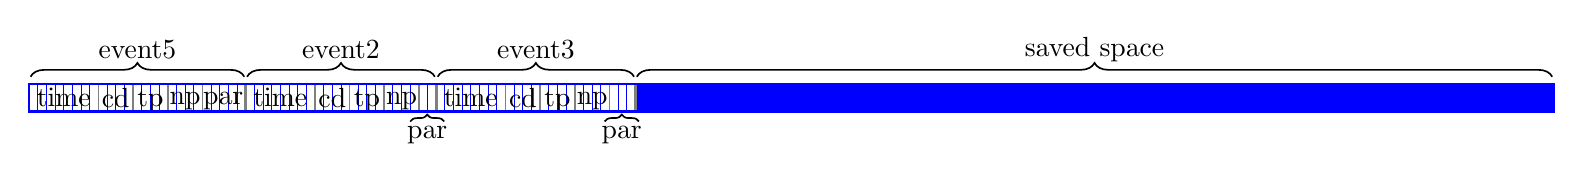
\begin{tikzpicture}[scale=.88]
    % vertical lines
    \foreach \x in {.125,.25,...,21.875}
        \draw[blue,line width=.12mm](\x,1.2) -- (\x,1.6);gray
    % event5
    \draw [
    semithick,
    decorate,
    decoration={
        brace,
        amplitude=5pt,
        raise=-0.35cm
    }] (0.02,2.1) -- (3.105, 2.1) node[midway]{event5}; 
    \draw (0.5, 1.4) -- (0.5, 1.4) node{time};
    \draw[gray,line width=.2mm](1.,1.2) -- (1.,1.6);
    \draw (1.25, 1.4) -- (1.25, 1.4) node{cd};
    \draw[gray,line width=.2mm](1.5,1.2) -- (1.5,1.6);
    \draw (1.75, 1.36) -- (1.75, 1.36) node{tp};
    \draw[gray,line width=.2mm](2.,1.2) -- (2.,1.6);  
    \draw (2.25, 1.35) -- (2.25, 1.35) node{np};
    \draw[gray,line width=.2mm](2.5,1.2) -- (2.5,1.6);
    \draw (2.8, 1.35) -- (2.8, 1.35) node{par};
    \draw[gray,line width=.4mm](3.125,1.2) -- (3.125,1.6);
    % event2
    \draw [
    semithick,
    decorate,
    decoration={
        brace,
        amplitude=5pt,
        raise=-0.35cm
    }] (3.145,2.1) -- (5.855, 2.1) node[midway]{event2};     
    \draw (3.625, 1.4) -- (3.625, 1.4) node{time};
    \draw[gray,line width=.2mm](4.125,1.2) -- (4.125,1.6);
    \draw (4.375, 1.4) -- (4.375, 1.4) node{cd};
    \draw[gray,line width=.2mm](4.625,1.2) -- (4.625,1.6);
    \draw (4.875, 1.36) -- (4.875, 1.36) node{tp};
    \draw[gray,line width=.2mm](5.125,1.2) -- (5.125,1.6);  
    \draw (5.375, 1.35) -- (5.375, 1.35) node{np};
    \draw[gray,line width=.2mm](5.625,1.2) -- (5.625,1.6);
    \draw [
    semithick,
    decorate,
    decoration={
        brace,
        amplitude=2.5pt,
        raise=-0.065cm
    }] (5.5,1.13) -- (5.99, 1.13) node[midway,below]{par}; 
    \draw[gray,line width=.4mm](5.875,1.2) -- (5.875,1.6);
    % event3
    \draw [
    semithick,
    decorate,
    decoration={
        brace,
        amplitude=5pt,
        raise=-0.35cm
    }] (5.895,2.1) -- (8.73, 2.1) node[midway]{event3};         
    \draw (6.375, 1.4) -- (6.375, 1.4) node{time};
    \draw[gray,line width=.2mm](6.875,1.2) -- (6.875,1.6);
    \draw (7.125, 1.4) -- (7.125, 1.4) node{cd};
    \draw[gray,line width=.2mm](7.375,1.2) -- (7.375,1.6);
    \draw (7.625, 1.36) -- (7.625, 1.36) node{tp};
    \draw[gray,line width=.2mm](7.875,1.2) -- (7.875,1.6);  
    \draw (8.125, 1.35) -- (8.125, 1.35) node{np};
    \draw[gray,line width=.2mm](8.375,1.2) -- (8.375,1.6);
    \draw [
    semithick,
    decorate,
    decoration={
        brace,
        amplitude=2.5pt,
        raise=-0.065cm
    }] (8.305,1.13) -- (8.8, 1.13) node[midway,below]{par};     
    \draw[gray,line width=.4mm](8.75,1.2) -- (8.75,1.6);
    % saved space
    \draw [
    semithick,
    decorate,
    decoration={
        brace,
        amplitude=5pt,
        raise=-0.35cm
    }] (8.77,2.1) -- (21.98, 2.1) node[midway]{saved space};
    % gray rectangle
    \draw [gray, fill=blue, line width=.12mm]
        (8.77,1.2) rectangle (22.,1.6);     
    % big rectangle
    \draw [blue, line width=.3mm]
        (0.,1.2) rectangle (22.,1.6);
           
    \end{tikzpicture}
}
  \end{footnotesize}  
\caption{Storage of different kinds of events in the trace file. 
In the figure, \emph{time} is the time when the event occurred; 
\emph{cd} means the event code; \emph{tp} is the event type; \emph{np} stands 
for the number of event's parameters; \emph{par}\dash{}an array of parameters.}
\label{fig:event_storage_all}
\end{center}
\end{figure}
